\textbf{Ejemplo 1}\\
Para realizar un proyecto se necesita realizar una inversión inicial de 80.000 COP y otra inversión de
45.000 COP al final del primer mes, en los meses 2 y 3 los ingresos son equivalentes a los egresos;
pero a partir del mes 4, se producen ingresos así: Mes cuatro 30.000 COP, mes cinco 50.000 COP, mes
seis 60.000 COP. Determinar si el proyecto lo pueden realizar los inversionistas A o B mencionados
anteriormente.\\


%%%%%%%%%%%%%%%%%%% EJERCICIO 1 %%%%%%

%\newpage %USAR SOLO SI EL SOLUCION QUEDA SOLO Y ES NECESARIO BAJARLO A LA SIGUIENTE PAGINA
\textbf{Solución.}\\
%La tabla ira centrada
\begin{center}
	\renewcommand{\arraystretch}{1.5}% Margenes de las celdas
	%Creacion de la cuadricula de 3 columnas \end{flushleft}
	\begin{longtable}[H]{|C{0.3\linewidth}|C{0.3\linewidth}|C{0.3\linewidth}|}
		%Creamos una linea horizontal
		\hline
         %%%%% INICIO FLUJO DE CAJA
		\rowcolor[HTML]{FFB183}
		\multicolumn{3}{|c|}{\cellcolor[HTML]{FFB183}\textbf{1. Asignación periodo focal}}   \\ \hline
		\multicolumn{3}{|c|} {$pf = 0 pmv$} \\ \hline
		%%%%%%%%%% FIN TITULO
		%%%%%%%%%% INICIO TITULO
		%Lo que se hace aqui es mezclar las 3 columnas en una sola
		\multicolumn{3}{|c|}{\cellcolor[HTML]{FFB183}\textbf{2. Declaración de variables}}   \\ \hline
		%%%%%%%%%% FIN TITULO
		%%%%%%%%%% INICIO DE MATEMATICAS
		%Cada & hace referencia al paso de la siguiente columna
		$n_{0} = 0 pmv$   & $n_{1} = 1 pmv$ & $n_{2} =  4 pmv$\\
		$n_{3} = 5 pmv$ & $n_{4} = 6 pmv$ & \\ \hline
		\multicolumn{3}{|c|}{$i_{a} = TIO_{a} = 3\% \equiv 0.03 pmv$} \\
		\multicolumn{3}{|c|}{$i_{b} = TIO_{b} = 2\% \equiv 0.02 pmv$} \\ \hline
		%%%%%%%%%% FIN DE MATEMATICAS
		%%%%% FIN DECLARACION DE VARIABLES


		%%%%% INICIO FLUJO DE CAJA
		\rowcolor[HTML]{FFB183}
		\multicolumn{3}{|c|}{\cellcolor[HTML]{FFB183}\textbf{3. Diagrama de flujo de caja}} \\ \hline
		%Mezclamos 3 columnas y ponermos el dibujo
		%%%%%%%%%%%%% INSERCION DE LA IMAGEN
		%Deberan descargar las imagenes respectivas del drive y pegarlas en la carpeta
		%n_capitulo/img/ejemplos/1/capitulo1ejemplo1.pdf  (el /1/ es el numero del ejemplo)
		\multicolumn{3}{|c|}{ 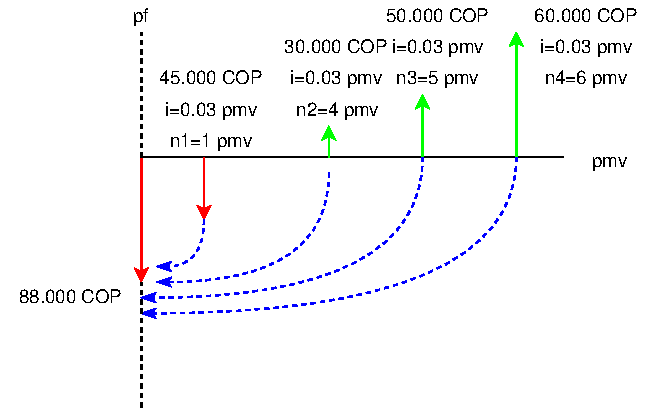
\includegraphics[trim=-5 -5 -5 -5 , scale=1.0,width=300px, height=250px]{9_Capitulo/ejemplos/1/Capitulo9Ejercicio1.pdf} }   \\ \hline
		%%%%%%%%%%%%% FIN INSERCION DE IMAGEN
		%%%%%FIN FLUJO DE CAJA



		%%%%% INICIO DECLARACION FORMULAS
		%%%%%%%%%%% INICIO TITULO
		\rowcolor[HTML]{FFB183}
		\multicolumn{3}{|c|}{\cellcolor[HTML]{FFB183}\textbf{4. Declaración de fórmulas}}    \\ \hline
		%%%%%%%%%%% FIN TITULO
		%%%%%%%%%%% INICIO MATEMATICAS
		\multicolumn{3}{|c|}{$\sum F_{n}(1+i)^{-n} $\hspace{0.3cm} \textit{Valor presente neto}} \\ \hline
		%%%%%%%%%% FIN MATEMATICAS
		%%%%%% INICIO DESARROLLO MATEMATICO
		\rowcolor[HTML]{FFB183}
		%%%%%%%%%%INICIO TITULO
		\multicolumn{3}{|c|}{\cellcolor[HTML]{FFB183}\textbf{5. Desarrollo matemático}}       \\ \hline
		%%%%%%%%%% FIN TITULO
		%%%%%%%%%% INICIO MATEMATICAS
		\multicolumn{3}{|c|}{$VPN_{a} = -80000 - 45000(1+0.03)^{-1} + 30000(1+0.03)^{-4} + 50000(1+0.03)^{-5} + 60000(1+0.03)^{-6}$} \\
		\multicolumn{3}{|c|}{$VPN_{a} = -3655$} \\
		\multicolumn{3}{|c|}{$VPN_{b} = -80000 - 45000(1+0.02)^{-1} + 30000(1+0.02)^{-4} + 50000(1+0.02)^{-5} + 60000(1+0.02)^{-6}$} \\
		\multicolumn{3}{|c|}{$VPN_{b} = 216254$} \\ \hline

		%%%%%%%%%% FIN MATEMATICAS
		%%%%%% FIN DESARROLLO MATEMATICO
		%%%%%% INICIO RESPUESTA
		\rowcolor[HTML]{FFB183}
		%%%%%%%%%%INICIO TITULO
		\multicolumn{3}{|c|}{\cellcolor[HTML]{FFB183}\textbf{6. Respuesta}}   \\ \hline
		%%%%%%%%%% FIN TITULO
		%%%%%%%%%% INICIO RESPUESTA MATEMATICA
		\multicolumn{3}{|c|}{Para B el $VPN > 0$, significa que puede realizar el proyecto en pesos de hoy,} \\ 
		\multicolumn{3}{|c|}{además de ganarse el 2\%, obtiene una ganancia de 2.162,54 COP.}  \\ \hline
		%%%%%%%%%% FIN MATEMATICAS
		%%%%%% FIN RESPUESTA
	\end{longtable}
	%Se crean dos lineas en blanco para que no quede el siguiente texto tan pegado
	%\newline \newline %USARLO SI CREES QUE ES NECESARIO
\end{center}
%%%%%%%%%%%%%%%%%%%%%%%%%%FIN EJERCICIO 1 %%%%%%%%%%%%%%%%%%%%%%%%%%%
